\documentclass{article}

\usepackage{graphicx}
\usepackage{sidecap}
\usepackage{caption}

\usepackage[a4paper,landscape,margin=1in]{geometry}

\begin{document}

\begin{SCfigure}[1][!ht]
  \captionsetup{labelformat=empty}
  \caption{
    Frame 1:
  }
  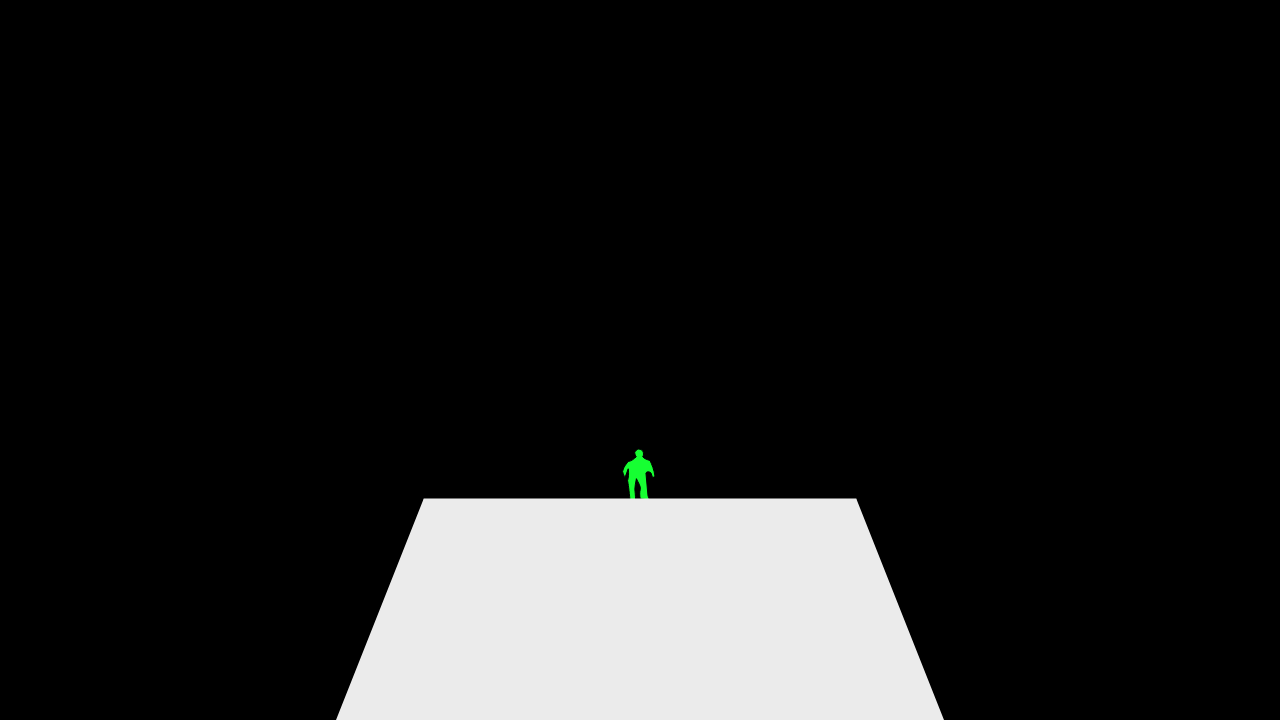
\includegraphics[width=0.5\textwidth]{Frame1.png}
\end{SCfigure}

\begin{SCfigure}[1][!ht]
  \captionsetup{labelformat=empty}
  \caption{
    Frame 2:
  }
  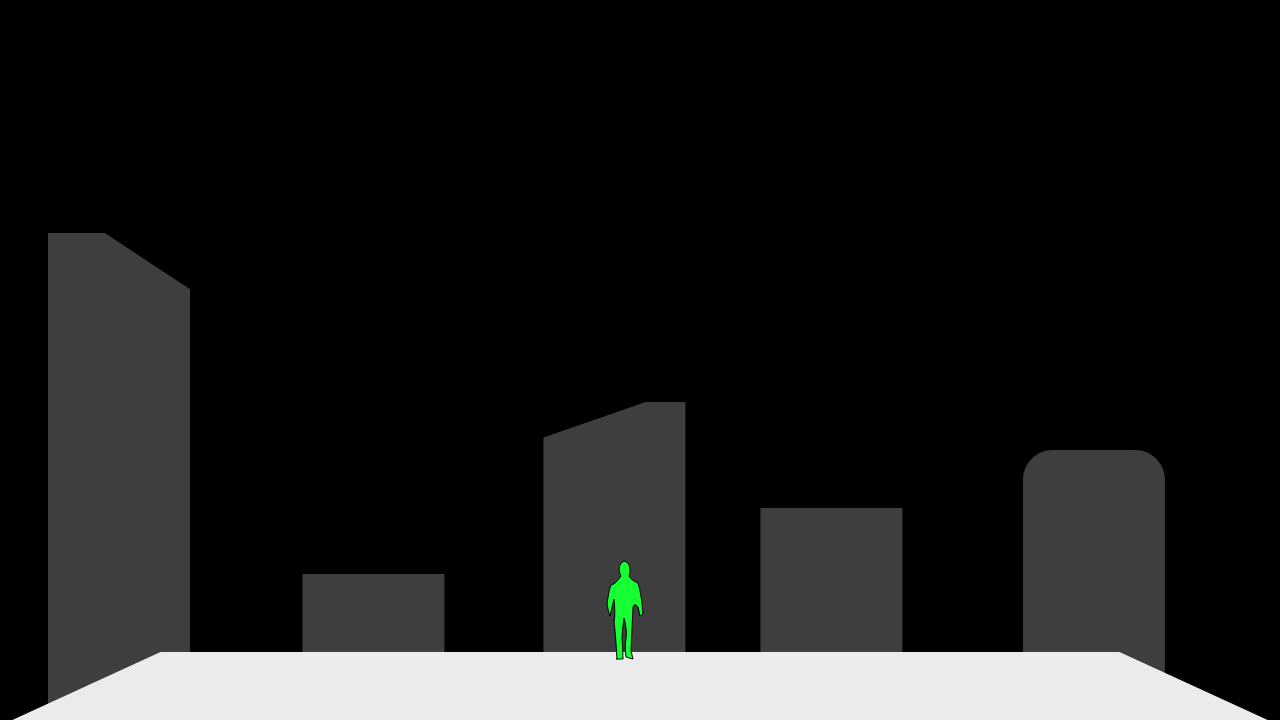
\includegraphics[width=0.5\textwidth]{Frame2.png}
\end{SCfigure}

\begin{SCfigure}[1][!ht]
  \captionsetup{labelformat=empty}
  \caption{
    Frame 3:
  }
  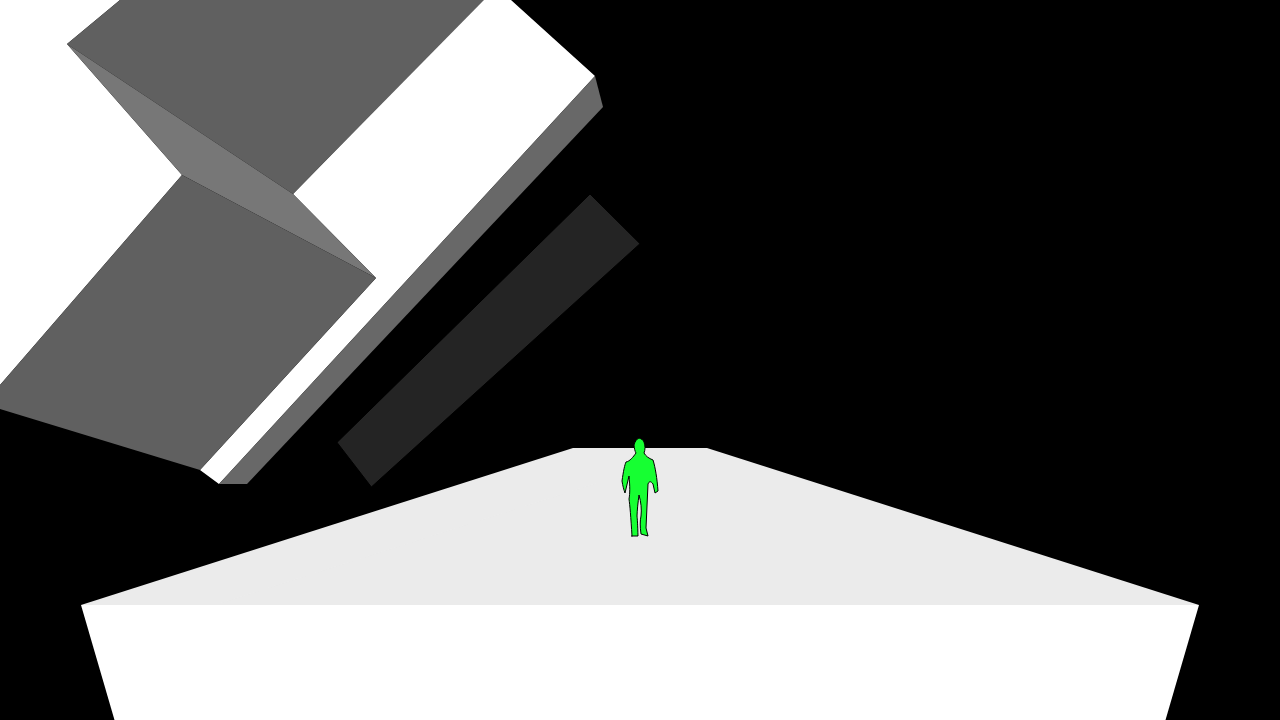
\includegraphics[width=0.5\textwidth]{Frame3.png}
\end{SCfigure}

\begin{SCfigure}[1][!ht]
  \captionsetup{labelformat=empty}
  \caption{
    Frame 4:
  }
  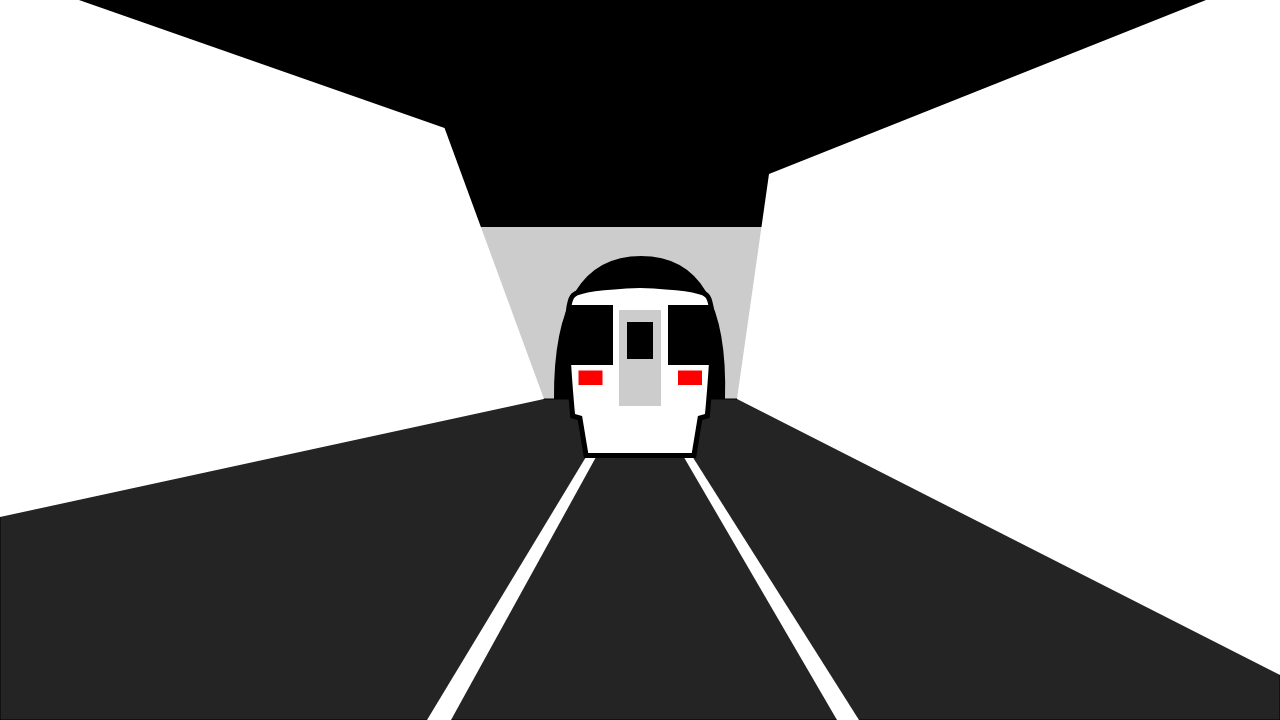
\includegraphics[width=0.5\textwidth]{Frame4.png}
\end{SCfigure}

\begin{SCfigure}[1][!ht]
  \captionsetup{labelformat=empty}
  \caption{
    Frame 5:
  }
  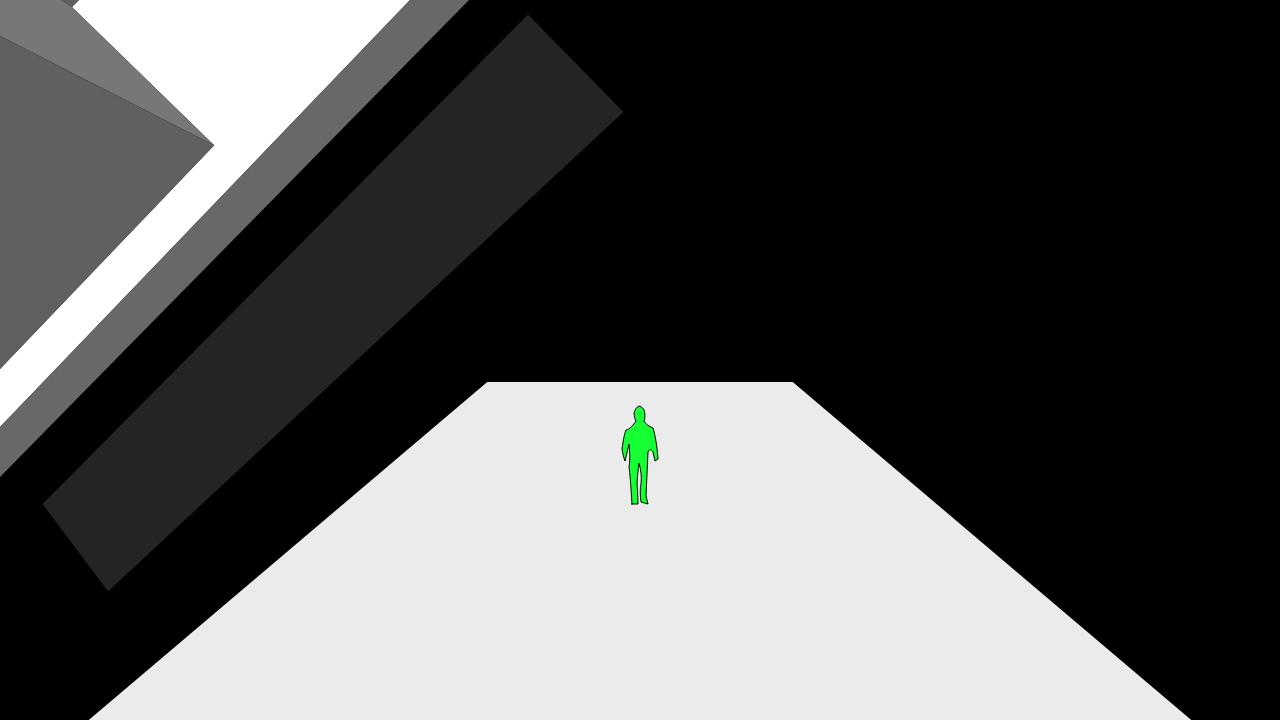
\includegraphics[width=0.5\textwidth]{Frame5.png}
\end{SCfigure}

\begin{SCfigure}[1][!ht]
  \captionsetup{labelformat=empty}
  \caption{
    Frame 6:
  }
  
\includegraphics[width=0.5\textwidth]{Frame6.png}
\end{SCfigure}

\begin{SCfigure}[1][!ht]
  \captionsetup{labelformat=empty}
  \caption{
    Frame 7:
  }
  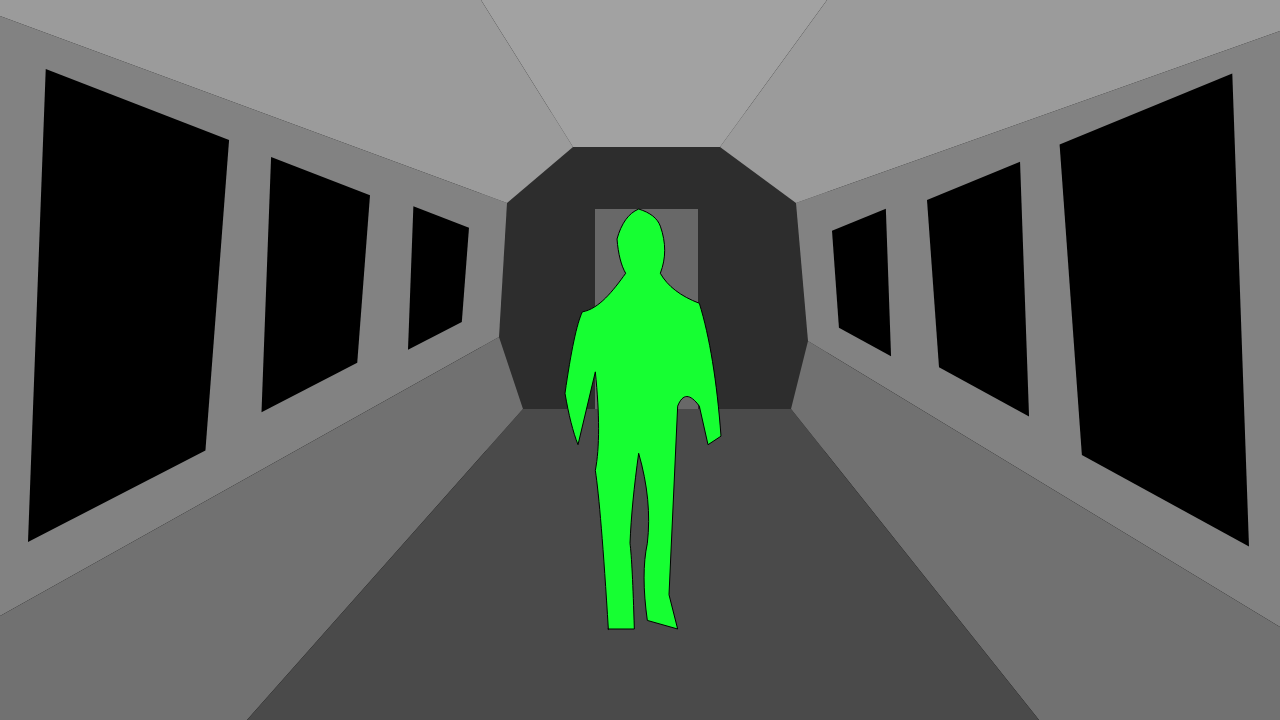
\includegraphics[width=0.5\textwidth]{Frame7.png}
\end{SCfigure}

\end{document}
